\documentclass[tikz,border=6pt]{standalone}
\usepackage[T1]{fontenc}
\usepackage{lmodern}
% arrows.meta 提供下面路径使用的 Latex 箭头样式，请勿删除。
\usetikzlibrary{arrows.meta}

% 在仓库根目录运行下面的命令重新生成图片：
% make -C paper figure-scirm

% ======================== 坐标与修改规则 ========================
% TikZ 坐标写成 (x,y)，单位默认为 cm。
% x 增大表示向右移动；本图中的 y 均为负数，y 越小表示越向下移动。
% node 的 at (x,y) 控制文字位置；draw 的起点和终点控制线条或外框范围。
% 修改可见文字后若发生换行，应同时检查 text width、外框高度和后续组件的 y。
% 字号从小到大依次为：\tiny、\scriptsize、\footnotesize、\small、\normalsize。

% ======================== 颜色组件 ========================
% HTML 色值采用 RRGGBB 格式，直接修改花括号中的六位字符即可换色。
% 组件颜色 1：正文与普通标题颜色。
\definecolor{ink}{HTML}{1A1A1A}
% 组件颜色 2：上方 prompt 外框和内部灰色分隔线。
\definecolor{rulegray}{HTML}{333333}
% 组件颜色 3：RF 标题、路径和 RF 输出框。
\definecolor{rfaccent}{HTML}{003B5C}
% 组件颜色 4：DS 标题、路径和 DS 输出框。
\definecolor{dsaccent}{HTML}{8B1E2D}
% 组件颜色 5：所有外框内部背景；FFFFFF 为纯白。
\definecolor{panelbg}{HTML}{FFFFFF}
% 若需要纯黑白版，将 rfaccent 和 dsaccent 都改为 222222。

% 该命令生成 [QUERY]、[CRITERIA]、[ANSWER] 等粗体字段名。
% 修改 ink 可统一换色；修改 \textbf 可取消粗体。
\newcommand{\field}[1]{\textcolor{ink}{\textbf{[#1]}}}

\begin{document}
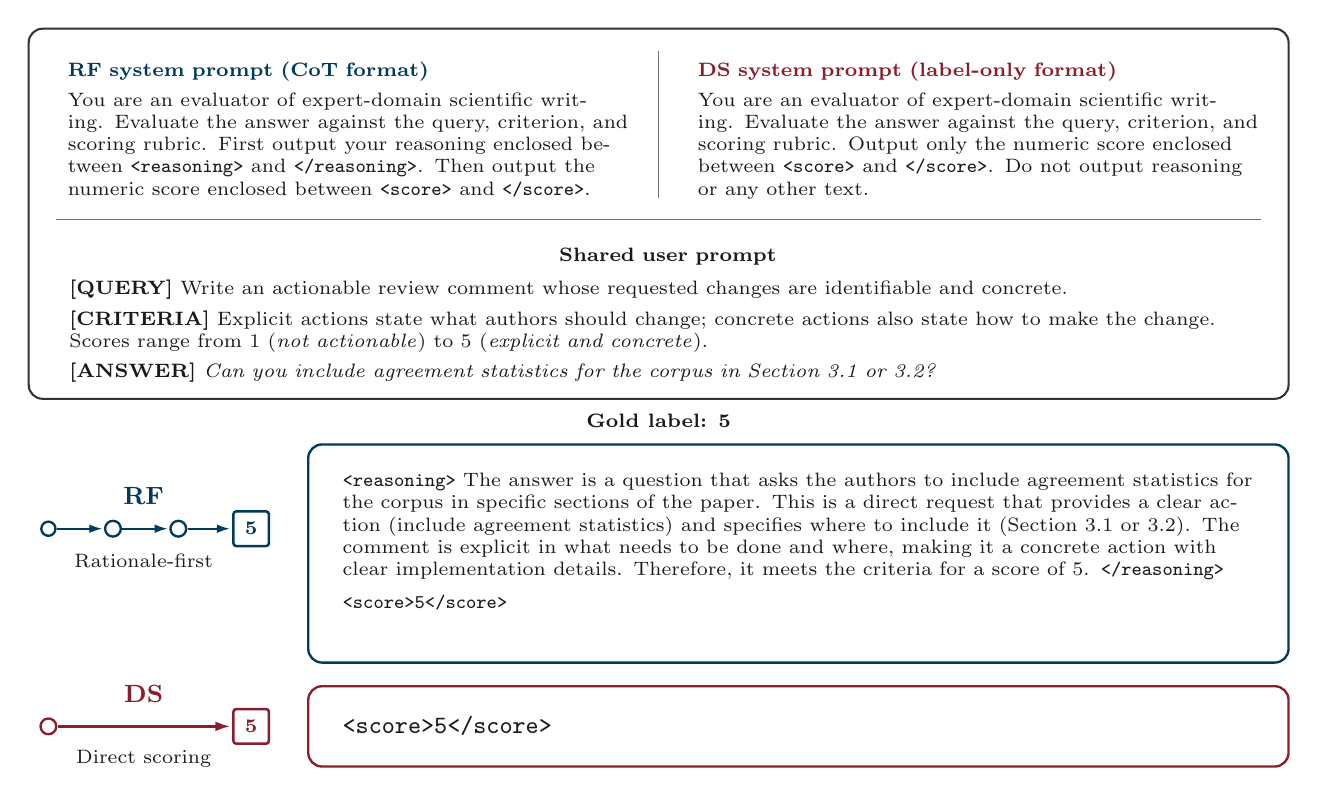
\begin{tikzpicture}[
  % 全局字体。将 \rmfamily 改为 \sffamily 可切换为无衬线字体。
  font=\rmfamily,
  % 所有文字默认使用 ink；outer sep=0pt 防止节点额外扩大画布。
  every node/.style={outer sep=0pt, text=ink}
]

% ======================== 上方 PROMPT 区域 ========================

% 组件 1：上方 prompt 总外框。
% 左上角为 (0,0)，右下角为 (16.0,-4.70)，因此宽 16.0、高 4.70。
% 修改右下角第一个数可改宽度，修改第二个数可改高度。
% line width 控制边框粗细；rounded corners 控制圆角大小；fill 控制背景。
\draw[draw=rulegray, fill=panelbg, line width=0.75pt, rounded corners=5pt]
  (0,0) rectangle (16.0,-4.70);

% 组件 2：RF 与 DS system prompt 之间的竖直分隔线。
% x=8.0 控制左右分栏比例；两个 y 控制线条的顶部和底部。
% x 变小会缩窄左侧 RF 区域，x 变大会缩窄右侧 DS 区域。
\draw[rulegray!70, line width=0.45pt] (8.0,-0.28) -- (8.0,-2.15);

% 组件 3：system prompt 与 shared user prompt 之间的水平分隔线。
% y=-2.42 控制上下区域比例；两端 x=0.35 和 x=15.65 控制左右留白。
% y 越接近 0，上方区域越矮；y 越小，上方区域越高。
\draw[rulegray!70, line width=0.45pt] (0.35,-2.42) -- (15.65,-2.42);

% 组件 4：左上方 RF system prompt 文本节点。
% at (0.38,-0.30) 是文本左上角；修改 x/y 可整体移动。
% text width=7.15cm 控制换行宽度；font 中的 \scriptsize 控制字号。
% 标题颜色由 rfaccent 控制；\par\vspace{3pt} 控制标题与正文间距。
\node[anchor=north west, align=left, text width=7.15cm,
      font=\rmfamily\scriptsize] at (0.38,-0.30) {%
  \textcolor{rfaccent}{\textbf{RF system prompt (CoT format)}}\par\vspace{3pt}
  You are an evaluator of expert-domain scientific writing. Evaluate the
  answer against the query, criterion, and scoring rubric. First output your
  reasoning enclosed between \texttt{<reasoning>} and
  \texttt{</reasoning>}. Then output the numeric score enclosed between
  \texttt{<score>} and \texttt{</score>}.
};

% 组件 5：右上方 DS system prompt 文本节点。
% at (8.38,-0.30) 是文本左上角；x 应保持在竖直分隔线 x=8.0 的右侧。
% text width=7.15cm 控制换行；若修改竖直分隔线，应同步调整 x 和 text width。
% 标题颜色由 dsaccent 控制；字号和标题间距的修改方法与组件 4 相同。
\node[anchor=north west, align=left, text width=7.15cm,
      font=\rmfamily\scriptsize] at (8.38,-0.30) {%
  \textcolor{dsaccent}{\textbf{DS system prompt (label-only format)}}\par\vspace{3pt}
  You are an evaluator of expert-domain scientific writing. Evaluate the
  answer against the query, criterion, and scoring rubric. Output only the
  numeric score enclosed between \texttt{<score>} and \texttt{</score>}.
  Do not output reasoning or any other text.
};

% 组件 6：下方 shared user prompt 文本节点。
% at (0.40,-2.67) 是文本左上角；text width=15.20cm 使其横跨整个外框。
% 修改 y 可整体上下移动；修改 text width 可调整右侧留白和换行位置。
% \centering 仅作用于标题，后面的 \raggedright 恢复正文左对齐。
\node[anchor=north west, align=left, text width=15.20cm,
      font=\rmfamily\scriptsize] at (0.40,-2.67) {%
  % 组件 6a：共享 user prompt 标题；vspace 控制标题与 QUERY 的距离。
  \centering\textbf{Shared user prompt}\par\vspace{4pt}
  \raggedright
  % 组件 6b：QUERY。替换字段后的英文即可，保留 \field 和结尾的间距命令。
  \field{QUERY} Write an actionable review comment whose requested changes are
  identifiable and concrete.\par\vspace{3pt}
  % 组件 6c：CRITERIA。文字变长时可能需要增大组件 1 的高度。
  \field{CRITERIA} Explicit actions state what authors should change; concrete
  actions also state how to make the change. Scores range from 1
  (\textit{not actionable}) to 5 (\textit{explicit and concrete}).\par\vspace{3pt}
  % 组件 6d：ANSWER。更换真实样例时，应同步修改组件 7、18、26 和论文图注。
  \field{ANSWER} \textit{Can you include agreement statistics for the corpus
  in Section 3.1 or 3.2?}
};

% 组件 7：gold label。
% at (8.0,-4.98) 控制中心位置；x=8.0 表示水平居中。
% 更换样例时修改数字 5，并同步修改 RF/DS 分数与图注。
\node[font=\rmfamily\scriptsize\bfseries] at (8.0,-4.98)
  {Gold label: 5};

% ======================== RF 协议与输出 ========================
% 真实来源：
% outputs/evaluations/rev_util_actionability/
% rev_util_actionability#qwen3_4b#base#greedy#on_cot#seed_base/
% predictions.jsonl，样例 actionability_test_0669。

% 组件 8：RF 缩写，位于多步路径上方。
% 箭头横向范围约为 x=0.36 到 x=2.56，中心是 x=1.46。
\node[text=rfaccent, font=\rmfamily\small\bfseries]
  at (1.46,-5.94) {RF};

% 组件 9：RF 路径的输入圆点。
% 圆心为 (0.25,-6.35)，circle (0.09) 中的 0.09 是半径。
\draw[rfaccent, line width=0.85pt]
  (0.25,-6.35) circle (0.09);

% 组件 10：RF 第一段箭头，从输入圆点指向第一个推理节点。
% 两个坐标控制起点和终点；Latex 的 length/width 控制箭头头部大小。
\draw[rfaccent, line width=0.85pt, -{Latex[length=1.7mm,width=1.1mm]}]
  (0.36,-6.35) -- (0.94,-6.35);

% 组件 11：RF 第一个中间推理节点；0.10 是圆点半径。
\draw[rfaccent, line width=0.85pt]
  (1.07,-6.35) circle (0.10);

% 组件 12：RF 第二段箭头，连接两个中间推理节点。
\draw[rfaccent, line width=0.85pt, -{Latex[length=1.7mm,width=1.1mm]}]
  (1.19,-6.35) -- (1.77,-6.35);

% 组件 13：RF 第二个中间推理节点。
\draw[rfaccent, line width=0.85pt]
  (1.90,-6.35) circle (0.10);

% 组件 14：RF 第三段箭头，从最后一个推理节点指向分数框。
% 若要拉长整条路径，应同时增大本箭头终点和组件 15 的两个 x。
\draw[rfaccent, line width=0.85pt, -{Latex[length=1.7mm,width=1.1mm]}]
  (2.02,-6.35) -- (2.56,-6.35);

% 组件 15：RF 路径末端的分数小框。
% 左下角为 (2.60,-6.57)，右上角为 (3.05,-6.13)。
% 修改两个 x 可移动/缩放宽度，修改两个 y 可移动/缩放高度。
\draw[draw=rfaccent, line width=0.9pt, rounded corners=1pt]
  (2.60,-6.57) rectangle (3.05,-6.13);

% 组件 16：RF 分数小框内的数字。
% at (2.825,-6.35) 是组件 15 的中心；移动小框时应同步修改。
\node[text=rfaccent, font=\rmfamily\scriptsize\bfseries]
  at (2.825,-6.35) {5};

% 组件 17：Rationale-first 小字，位于路径下方。
% at (1.46,-6.76) 位于箭头本身的水平中心，而不是整个路径的中心。
\node[font=\rmfamily\scriptsize]
  at (1.46,-6.76) {Rationale-first};

% 组件 18：RF 右侧输出外框。
% 左上相关坐标为 x=3.55、y=-5.28，右下角为 (16.0,-8.05)。
% 减小 3.55 会让框向左扩展；增大则向右收窄。
% 修改 y=-5.28/-8.05 可调整框的顶部、底部和高度。
\draw[draw=rfaccent, fill=panelbg, line width=0.85pt, rounded corners=5pt]
  (3.55,-5.28) rectangle (16.0,-8.05);

% 组件 19：RF 输出文字。
% at (3.87,-5.53) 比外框左/上边各留约 0.32/0.25 cm。
% text width=11.65cm 控制换行；外框左移时可以增大，右移时必须减小。
% 更换真实输出时替换节点内部文字，并保留 reasoning/score 标签格式。
\node[anchor=north west, align=left, text width=11.65cm,
      font=\rmfamily\scriptsize] at (3.87,-5.53) {%
  \textbf{\texttt{<reasoning>}} The answer is a question that asks the authors
  to include agreement statistics for the corpus in specific sections of the
  paper. This is a direct request that provides a clear action (include
  agreement statistics) and specifies where to include it (Section 3.1 or
  3.2). The comment is explicit in what needs to be done and where, making it
  a concrete action with clear implementation details. Therefore, it meets the
  criteria for a score of 5. \textbf{\texttt{</reasoning>}}\par\vspace{4pt}
  \textbf{\texttt{<score>5</score>}}
};

% ======================== DS 协议与输出 ========================
% 真实来源：
% outputs/evaluations/rev_util_actionability/
% rev_util_actionability#qwen3_4b#base#greedy#on_label_only#seed_base/
% predictions.jsonl，样例 actionability_test_0669。

% 组件 20：DS 缩写，位于直达路径上方。
% 箭头横向范围约为 x=0.37 到 x=2.56，中心约为 x=1.46。
\node[text=dsaccent, font=\rmfamily\small\bfseries]
  at (1.46,-8.45) {DS};

% 组件 21：DS 路径的输入圆点。
% 圆心为 (0.25,-8.86)，circle (0.10) 中的 0.10 是半径。
\draw[dsaccent, line width=0.85pt]
  (0.25,-8.86) circle (0.10);

% 组件 22：DS 直达箭头，从输入圆点直接指向分数框。
% 路径由 x=0.37 延伸到 x=2.56；增大终点可拉长箭头。
% 拉长时应同步右移组件 23、24，并确保仍位于组件 25 左侧。
\draw[dsaccent, line width=0.9pt, -{Latex[length=1.9mm,width=1.25mm]}]
  (0.37,-8.86) -- (2.56,-8.86);

% 组件 23：DS 路径末端的分数小框。
% 左下角为 (2.60,-9.08)，右上角为 (3.05,-8.64)。
\draw[draw=dsaccent, line width=0.9pt, rounded corners=1pt]
  (2.60,-9.08) rectangle (3.05,-8.64);

% 组件 24：DS 分数小框内的数字。
% at (2.825,-8.86) 是组件 23 的中心；移动小框时应同步修改。
\node[text=dsaccent, font=\rmfamily\scriptsize\bfseries]
  at (2.825,-8.86) {5};

% 组件 25：Direct scoring 小字，位于路径下方。
% at (1.46,-9.27) 位于箭头本身的水平中心，而不是整个路径的中心。
\node[font=\rmfamily\scriptsize]
  at (1.46,-9.27) {Direct scoring};

% 组件 26：DS 右侧输出外框。
% 左边界 x=3.55 与 RF 外框对齐；右边界 x=16.0。
% y=-8.35/-9.37 控制顶部、底部和高度。
\draw[draw=dsaccent, fill=panelbg, line width=0.85pt, rounded corners=5pt]
  (3.55,-8.35) rectangle (16.0,-9.37);

% 组件 27：DS 输出文字。
% at (3.87,-8.86) 比外框左侧留 0.32 cm；anchor=west 表示垂直居中。
% 更换真实输出时直接替换标签内容；移动外框时应同步修改 x。
\node[anchor=west, font=\ttfamily\small\bfseries] at (3.87,-8.86)
  {<score>5</score>};

\end{tikzpicture}
\end{document}
